
%\begin{frame}[fragile]{Notation}
%    We defined \intracfgs\ using the RAGs formalism.
%
% \begin{onlyenv}<1>
%\phantom{test}\\
%\phantom{test}\\
%\phantom{test}\\
%\phantom{test}
% \end{onlyenv}
%
%
% \begin{onlyenv}<2>
%\begin{lstlisting}[language=JastAdd]
%syn int B.v() = 5;
%syn int C.v() = 2;
%syn int A.sum() = B.v() + C.v();
%\end{lstlisting}
%\phantom{test}
% \end{onlyenv}
%
% \begin{onlyenv}<3>
%\begin{lstlisting}[language=JastAdd]
%inh int B.v_p(); inh int C.v_p();
%eq A.getB().v_p() = A.getC().v_p();
%eq A.getC().v_p() = A.getB().v_p();
%\end{lstlisting}
%\phantom{test}
% \end{onlyenv}
%
% \begin{onlyenv}<4>
%\begin{lstlisting}[language=JastAdd]
%syn nta C.D() = new D();
%\end{lstlisting}
%\phantom{test}\\
%\phantom{test}
% \end{onlyenv}
%
% \begin{onlyenv}<5>
%\begin{lstlisting}[language=JastAdd]
%coll Set<ASTNode>  A.allChildren() [new HashSet<ASTNode>()] root A
%B contributes this to A.allChildren();
%C contributes this to A.allChildren();
%D contributes this to A.allChildren();
%\end{lstlisting}
% \end{onlyenv}
%
% \begin{onlyenv}<6>
%\begin{lstlisting}[language=JastAdd]
%syn Set<int> A.x() circular [new HashSet<>()]{
%  Set<int> res = new HashSet<int>(x);
%  if( flag ) res.add(x().size() +1);
%  return res; }
%\end{lstlisting}
% \end{onlyenv}
%
%    \begin{minipage}[h]{0.5\textwidth}
%        \only<1> {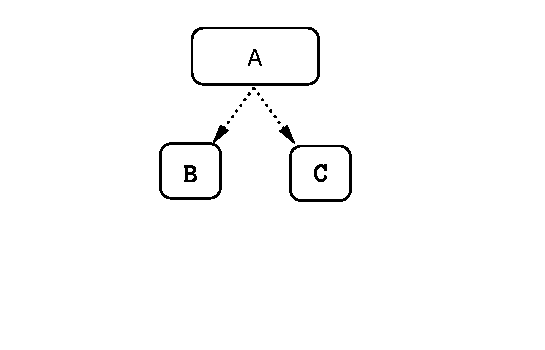
\includegraphics[scale=0.7]{img/ex1.pdf}}%
%        \only<2> {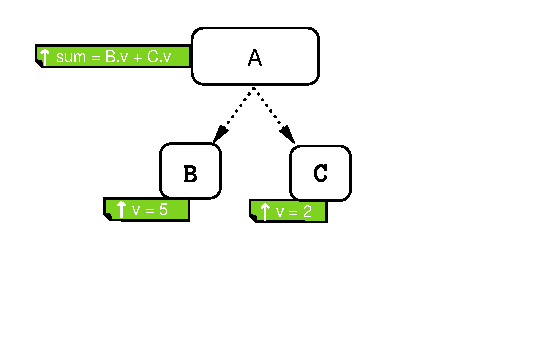
\includegraphics[scale=0.7]{img/ex2.pdf}}%
%        \only<3> {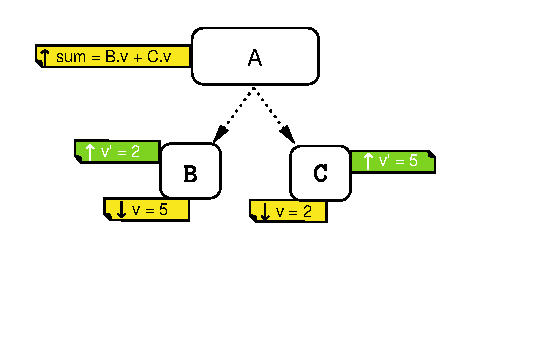
\includegraphics[scale=0.7]{img/ex3.pdf}}%
%        \only<4> {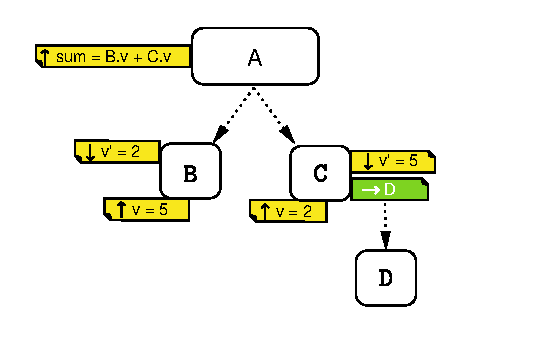
\includegraphics[scale=0.7]{img/ex4.pdf}}%
%        \only<5> {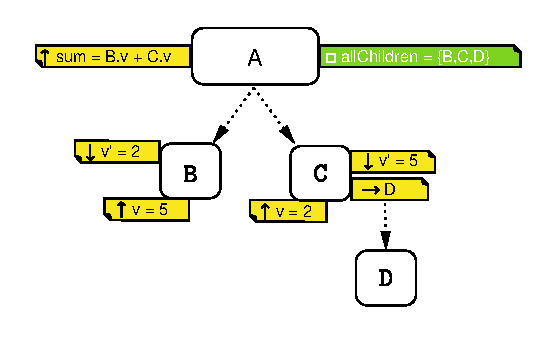
\includegraphics[scale=0.7]{img/ex5.pdf}}%
%		  \only<6-> {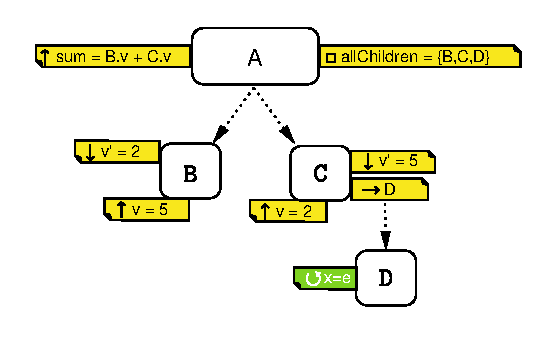
\includegraphics[scale=0.7]{img/ex6.pdf}}%
%    \end{minipage}\quad\quad\quad
%    \begin{minipage}[h]{0.3\textwidth}
%        \vspace*{-0.8cm}
%        \begin{table}[]
%            \begin{tabular}{l|l}
%            \textsc{Attribute}   & \textsc{Notation} \pause \\
%            \hline
%            \texttt{Synthesized} & \Asyn{x}=e \pause\\
%            \hline
%            \texttt{Inherited}   & \Ainh{x}=e \pause \\
%            \hline
%            \texttt{HOA}         & \Ahoa{x}=e \pause \\
%            \hline
%            \texttt{Collection}  & \Acoll{x} \pause \\
%            \hline
%            \texttt{Circular}  & \Acirc{x}=e
%            \end{tabular}
%            \end{table}
%    \end{minipage}%
%
%%\captionsetup{labelformat=empty}
%%\begin{block}{Jastadd Syntax}
%%\texttt }
%%\end{block}
%
%\end{frame}